% Put between [ ] in document class report type following these macros:
%
% + daily
% + weekly
% + monthly

\documentclass[daily]{engenius}

% Fill the document parameters
% Remove \titletwo if you want one title
% You can remove authors by deleting then
% You have 3 option for the department identification as showed bellow

\title{Pharma Comp.}
\titletwo{<<Product name/denomination>>}

% Use the author section to show some basic numbers
\author{Num. alerts \\ NUMBER
	\and Good batches percentage \\ NUMBER
    \and Bad batches count \\ NUMBER
    } 
    
\date{\today}
\version{0.0.1}

\begin{document}

\maketitle

\begin{abstract}

% Use the following placeholders as appropiate
% {<<BATCHES>>}
% {<<PERIOD_TYPE>>}
% {<<GOOD_BATCHES>>}
% {<<NUM_ALERTS>>}
% {<<BAD_BATCHES>>}
% {<<TOTAL_BATCHES>>}

% {<<PERC_GOOD_BATCHES>>}
% {<<PERC_OKAY_BATCHES>>}
% {<<PERC_BAD_BATCHES>>}

% {<<HIGHEST_TEMPERATURE>>}
% {<<LOWEST_TEMPERATURE>>}
% {<<HIGHEST_HUMIDITY>>}
% {<<LOWEST_HUMIDITY>>}
% {<<HIGHEST_UV_LIGHT>>}
% {<<LOWEST_UV_LIGHT>>}


% Replace the \textbf{WORD} with the corresponding placeholder


The report includes information for the batches \textbf{BATCHES}, up to the given date. For the \textbf{PERIOD\_TYPE} period, \textbf{NUM\_ALERTS} were triggered. Up to this data, \textbf{GOOD\_BATCHES} batches are predicted to be in good condition and \textbf{BAD\_BATCHES} in bad condition, from the \textbf{TOTAL\_BATCHES} total batches.

\end{abstract}

%%--------------------%%

\section{Categories per batch}
The model predicts the following classes for the given \textbf{TOTAL\_BATCHES} in the period.

% Show graphics of the classification of the different batches
\begin{figure}[!ht]
    \begin{center}
        % Modify direction of the imgs -> images directory
        
\includegraphics[width=\textwidth/3]{../images/logo2.png}
        \caption{Batch classification}
        \label{img:engeniuslogo}
    \end{center}
\end{figure}

According to model classification, \textbf{PERC\_GOOD\_BATCHES}\% have been handled well, \textbf{PERC\_OKAY\_BATCHES}\% have had a decent-okay handling, and \textbf{PERC\_BAD\_BATCHES}\% have been mistreated or have suffered some mishap during their journey.

%%--------------------%%

\section{Historical data}
\subsubsection{Temperature}

The temperature average of all the batches during the period was, as the next figure shows.

% Show plot of the temperature average over time
\begin{figure}[!ht]
    \begin{center}
        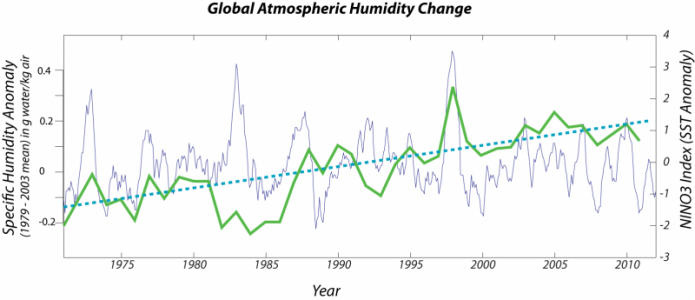
\includegraphics[width=\textwidth/3]{../images/humidity_example.png}
        \caption{Temperature over time}
        \label{img:engeniuslogo}
    \end{center}
\end{figure}

%%--------------------%%

\subsubsection{Humidity}

The humidity average of all the batches during the period was, as the next figure shows.

% Show plot of the temperature average over time
\begin{figure}[!ht]
    \begin{center}
        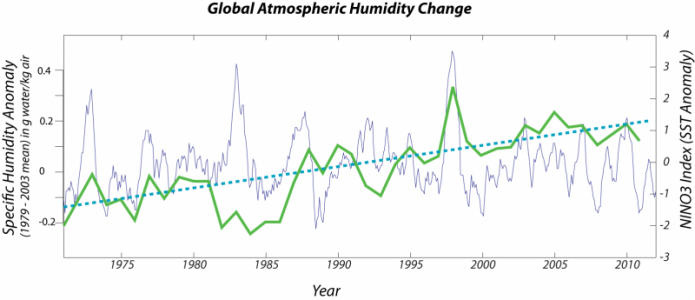
\includegraphics[width=\textwidth/3]{../images/humidity_example.png}
        \caption{Humidity over time}
        \label{img:engeniuslogo}
    \end{center}
\end{figure}

%%--------------------%%

\subsubsection{UV Light}

The UV light average of all the batches during the period was, as the next figure shows.

% Show plot of the temperature average over time
\begin{figure}[!ht]
    \begin{center}
        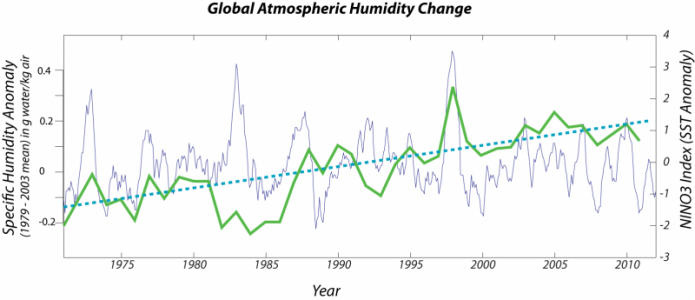
\includegraphics[width=\textwidth/3]{../images/humidity_example.png}
        \caption{UV Light over time}
        \label{img:engeniuslogo}
    \end{center}
\end{figure}

%%--------------------%%

\subsection{Notable Data Points}

The highest and lowest values for the temperature, humidity, and UV light for the day, amongst all batches, are as follows:

\begin{itemize}
    \item \textbf{Temperature:} Highest - \textbf{<<Highest\_Temperature>>}, Lowest - \textbf{<<Lowest\_Temperature>>}
    \item \textbf{Humidity:} Highest - \textbf{<<Highest\_Humidity>>}, Lowest - \textbf{<<Lowest\_Humidity>>}
    \item \textbf{UV Light:} Highest - \textbf{<<Highest\_UV\_Light>>}, Lowest - \textbf{<<Lowest\_UV\_Light>>}
\end{itemize}

%%--------------------%%

\subsection{Individual batches}

\subsubsection{Monitored Batches' Position}

The next table shows the approximate location of the batches monitored during the day.

\begin{table}[ht]
    \centering
    \begin{tabular}{|c|c|}
        \hline
        \textbf{Batch Number} & \textbf{Approximate Location} \\
        \hline
        001 & <<Location 001>> \\
        002 & <<Location 002>> \\
        \hline
        % Add more rows as needed
    \end{tabular}
    \caption{Approximate Locations of Monitored Batches}
    \label{tab:batch_positions}
\end{table}

%%--------------------%%

\subsubsection{Monitored Batches' Cumulative Transport Time}

The next table shows an approximation of the time that each batch has been on transport, starting from the moment the censoring module was installed, until now.

\begin{table}[ht]
    \centering
    \begin{tabular}{|c|c|}
        \hline
        \textbf{Batch Number} & \textbf{Transport time} \\
        \hline
        001 & <<Time 001>> \\
        002 & <<Time 002>> \\
        \hline
        % Add more rows as needed
    \end{tabular}
    \caption{Approximate Locations of Monitored Batches}
    \label{tab:batch_positions}
\end{table}


%% We may add a section for quick recomendations of action, based on the results of the report

\end{document}
